\documentclass[handout]{beamer}
\mode<presentation>
{
  \usetheme{Warsaw}
  \definecolor{acmblue}{rgb}{0.2, 0.4, 0.6}
  \definecolor{acmgray}{rgb}{0.1, 0.1, 0.1}
  \setbeamercolor{structure}{fg=acmblue,bg=acmgray}
  %\setbeamercovered{transparent}
}


\usepackage[english]{babel}
\usepackage[latin1]{inputenc}
\usepackage{times}
\usepackage[T1]{fontenc}
\usepackage{tikz}
\usepackage{graphicx}

\newcommand{\imagesource}[1]{{\centering\hfill\break\hbox{\scriptsize Image Source:\thinspace{\small\itshape #1}}\par}}

\title{2019 Fall Conference}


\author{ACM Mid-Southeast}

\date[]{}
\subject{}

\pgfdeclareimage[height=1.5cm]{university-logo}{acmlogo}
\logo{\pgfuseimage{university-logo}}



\begin{document}

\begin{frame}
  \begin{center}
    {\color{acmblue}\Huge ACM Mid-Southeast
        \vspace{0.5cm}
        \newline 2019 Fall Conference} 
    \newline
\includegraphics[height=0.5\textheight]{colorlogo}
  \end{center}
\end{frame}


% Structuring a talk is a difficult task and the following structure
% may not be suitable. Here are some rules that apply for this
% solution: 

% - Exactly two or three sections (other than the summary).
% - At *most* three subsections per section.
% - Talk about 30s to 2min per frame. So there should be between about
%   15 and 30 frames, all told.

% - A conference audience is likely to know very little of what you
%   are going to talk about. So *simplify*!
% - In a 20min talk, getting the main ideas across is hard
%   enough. Leave out details, even if it means being less precise than
%   you think necessary.
% - If you omit details that are vital to the proof/implementation,
%   just say so once. Everybody will be happy with that.


\begin{frame}{Schedule}
    \begin{description}
        \item[8:00 -- 8:10 a.m.] Welcome/Announcements -- Azalea
        \item[8:10 -- 9:00 a.m.] Keynote Address
        \item[9:00 -- 9:15 a.m.] Coffee Break -- Poolside
        \item[9:15 -- 10:35 a.m.] Session I
        \item[10:40 -- 12:00 p.m.] Session II
        \item[12:00 -- 1:00 p.m.] Lunch -- Patio Restaurant
        \item[1:00 -- 2:20 p.m.] Session III
        \item[2:20 -- 2:35 p.m.] Break -- Poolside
        \item[2:35 -- 3:55 p.m.] Session IV
        \item[4:30 -- 5:00 p.m.] Business Meeting -- Highlander I
        \item[5:00 -- 7:00 p.m.] Social Gathering, Hospitality Suite (235)
        \item[7:00 -- 8:30 p.m.] Awards Banquet -- Azalea
    \end{description}
\end{frame}

\begin{frame}{Room Layout}
    \begin{center}
        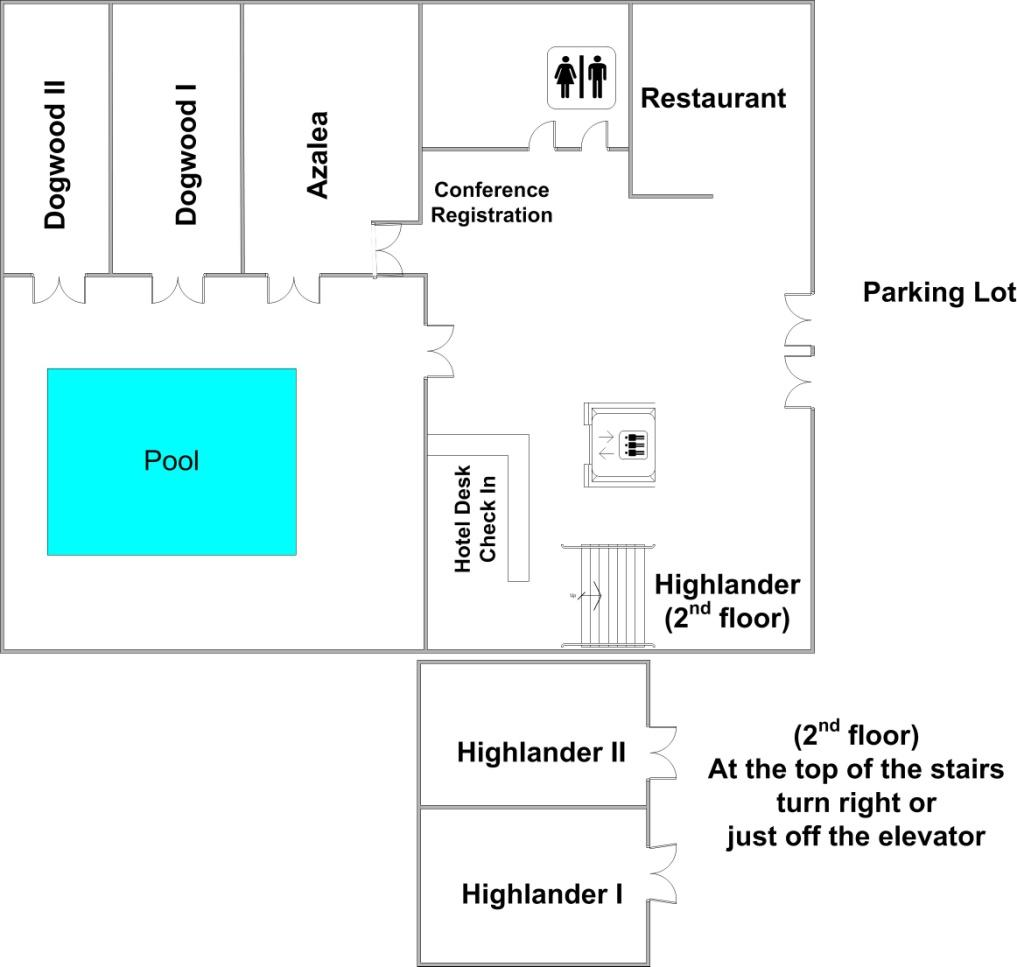
\includegraphics[height=0.85\textheight]{floorplan}
    \end{center}
\end{frame}

\begin{frame}{Session Guidelines}
    \textbf{Presenters}
    \begin{itemize}
        \item Arrive at your room 5 minutes before the beginning of
            your session to load your presentations on the room's
            laptop.
    \end{itemize}

    \textbf{Session Chairs}
    \begin{itemize}
        \item Introduce each speaker by name and institution.
        \item Give your speakers a five minute warning as they near
            the end of their time.
        \item Keep presentations in their assigned time slots. (Please do not
            start a presentation early.)
    \end{itemize}

    \textbf{Judges}
    \begin{itemize}
        \item Make sure you have your judging forms.
        \item Judges will meet at 4:00 in the restaurant.
    \end{itemize}
\end{frame}

\begin{frame}{Lunch and Banquet Tickets}
    \begin{columns}
    \column{0.5\textwidth}
    \begin{itemize}
        \item If you have a lunch or buffet ticket you do not plan to
            use, please give it to Bob Bradley after the keynote address.
    \end{itemize}
    \column{0.5\textwidth}
    \begin{center}
        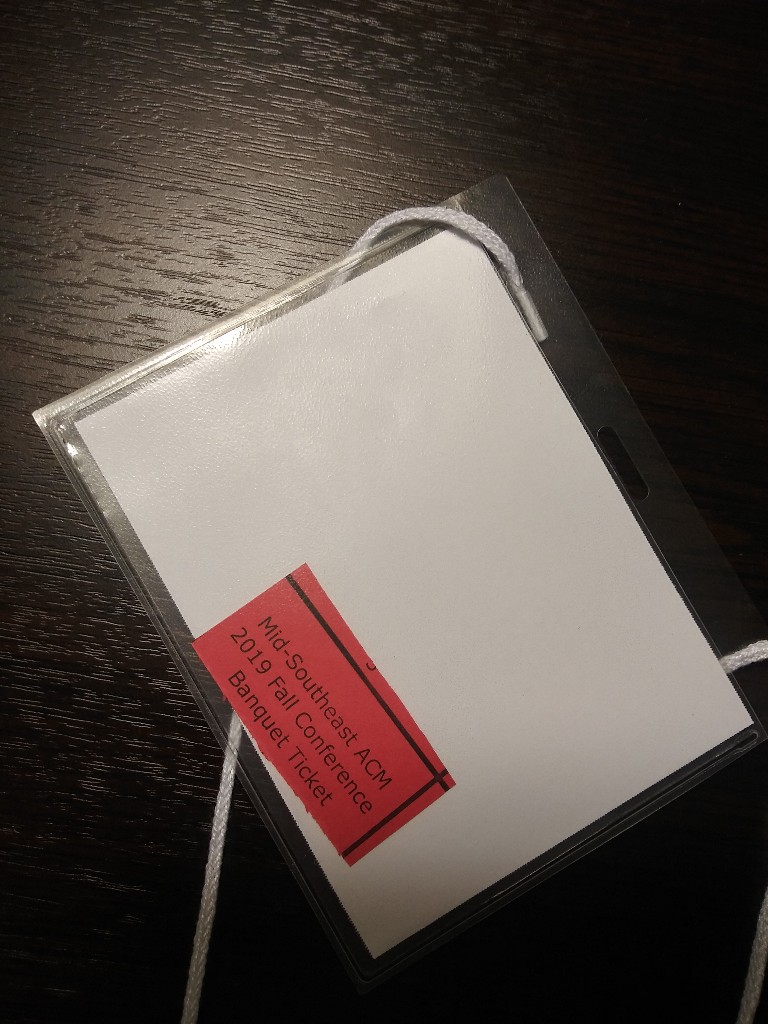
\includegraphics[width=0.8\textwidth]{banquet}
    \end{center}
    \end{columns}
\end{frame}

\begin{frame}{Program Changes}
    \begin{center}
        {\color{acmblue}\Huge Program Changes}
    \end{center}
\end{frame}

\begin{frame}{About Our Speaker}
\begin{columns}
    \column{0.7\textwidth}
    \textbf{Joseph Hagerman}
    \begin{itemize}
        \item Bachelor of Architecture from Mississippi State University
        \item MS in Civil Engineering from Columbia University
        \item Project Manager for the Building Technologies group at
            the Federation of America Scientists
        \item Senior Advisor to Assistant Secretary of DOE EERE
        \item Joins ORNL as National Rural Electric Cooperative Association's
            Deputy Chief Scientist
    \end{itemize}
    \column{0.3\textwidth}
    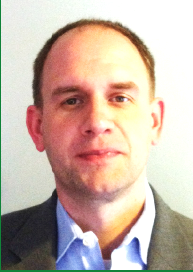
\includegraphics[width=0.9\textwidth]{hagerman}
\end{columns}
\end{frame}
\end{document}


